\chapter{Finding driver mutations} \label{chap:finding_driver_mutations}

% Although the true explanation for mutual exclusivity remains unknown, and its therapeutic potential is still uncertain, this phenomenon is frequently observed in data and may lead to discoveries in cancer treatment.

In the previous chapter, various studies were discussed in terms of how they formalized biological assumptions, with particular emphasis on the metrics developed to assess \textit{coverage} and \textit{mutual exclusivity} within gene groups. This chapter will delve deeper into the algorithms employed by these studies to identify driver pathways using their respective metrics and hypotheses.

Existing approaches can be categorized into two types: \textbf{\textit{de novo}} approaches, which identify mutually exclusive patterns using only genomic data from patients, and \textbf{\textit{knowledge-based}} methods, which integrate the analysis with external \textit{a priori} information. \textit{De novo} approaches might lack sufficient information as they do not utilize pre-existing pathway databases, protein-protein interaction (PPI) networks or phenotype data. Conversely, given that our understanding of gene and protein interactions in humans is still incomplete, and many pathway databases fail to accurately represent the specific pathways and interactions present in cancer cells, \textit{knowledge-based} approaches may be limited by their dependence on existing data sources. Consequently, \textit{de novo} methods might yield new but potentially less accurate results, while \textit{knowledge-based} approaches may limit the discovery of novel biological insights \cite{survey, multi-dendrix}.

\section{Dendrix}

\subsection{A greedy approach} \label{dendrix_first_sub}

\textcite{dendrix} introduced the most widely adopted metric in pathway discovery research, namely $W(M)$ (presented in \cref{weight}). In addition to this, they defined the Maximum Weight Submatrix Problem (MWSP), discussed in \cref{mwsp}, and proposed the following \textit{greedy algorithm}, called Dendrix (\textit{de novo} \cite{survey}), to solve it.

\begin{algorithm}[H]
    \caption{
        \textit{Greedy Dendrix}: given the set of all genes $\mathcal G$, and an integer $k$, the algorithm finds the set of genes $M$ of size $k$ that maximizes $W(M)$.
    }

        \label{greedy_dendrix}
    \begin{algorithmic}[1]
        \Function{greedyDendrix}{$\mathcal G$, $k$}
            \State $M := \{g_1, g_2\}$ such that $M$ maximizes $W(M)$ \Comment{pick the best gene pair}
            \For{$i \in [3, k]$}
                \State $\hat g := \argmax_{g \in \mathcal G}{W \rbk{M \cup \{g\}}}$ \Comment{TODO \href{http://web.archive.org/web/20220805140851/https://compbio.cs.brown.edu/software/}{SOURCE} PER PARIM?}
                \State $M = M \cup \{\hat g\}$
            \EndFor
            \State \textbf{return} $M$
        \EndFunction
    \end{algorithmic}
\end{algorithm}

Clearly, the time complexity of the algorithm is $O\rbk{n^2 + kn} = O\rbk{n^2}$ --- where $n = \abs{\mathcal G}$, therefore $k \le n$ --- because finding $\{g_1, g_2\}$ in line 2 requires $O\rbk{n^2}$ and the $\argmax{}$ in line 4 has cost $O(n)$. 

While this algorithm is efficient, there is generally no guarantee that it will identify the optimal set $\hat M$ that maximizes $W(\hat M)$. However, \textcite{dendrix} prove that \cref{greedy_dendrix} can correctly identify $\hat M$ with high probability when the mutation data come from the \textit{Gene Independence Model} (GIM), which is described below. \todo{ne forniscono una dimostrazione nel materiale supplementare, ma è lunga 3 pagine, e non credo sia oppurtuno inserire una cosa cosi lunga qui, penso che sia \curlyquotes{beyond the scope}}

\begin{definition}[Gene Independence Model] \todo{capire bene questo modello}
    Let $A$ be an $m \times n$ mutation matrix, such that $\hat M$ is the \textit{maximum weight submatrix} of $A$, and $|\hat M| = k$; the matrix $A$ satisfies the \textbf{Gene Independence Model} (GIM) if and only if:

    \begin{enumerate}[label=\roman*), font=\itshape]
        \item each gene $g \notin \hat M$ is mutated in each patient with probability $p_g \in \sbk{p_L, p_U}$ \todo{WHAT ARE THESE??}, independently of all other events;
        \item $W (\hat M)= \Omega(m)$; \todo{qua scrivono che la definizione di $Omega$ è che $W (\hat M) = rm$ per $0 < r \le 1$???????}
        \item for all $M \subset \hat M$ of cardinality $l := \abs{M}$, it exists $0 \le d < 1$ such that $$W(M) \le \frac{l + d}{k} W(\hat M)$$
    \end{enumerate}
\end{definition}

Note that:

\begin{itemize}
    \item condition $(i)$ reflects the independence of mutations for genes outside the mutated pathway, a standard assumption for somatic single-nucleotide mutations, according to \textcite{dendrix};
    \item condition $(ii)$ ensures that mutations in $\hat M$ cover a large number of patients and are mostly exclusive;
    \item condition $(iii)$ means that each gene in $\hat M$ is important, so there are no subset of $\hat M$ that predominantly contributes to $W(\hat M)$.
\end{itemize}

Although it is possible to efficiently obtain accurate results with high probability under the GIM, genes within $\hat M$ may exhibit \textit{observed mutation frequencies} similar to those of genes outside $\hat M$. This similarity can make it challenging to distinguish between them based solely on mutation frequency, regardless of the number of patients.

To illustrate this, consider the following scenario: observed gene mutation frequencies fall within the range of $[3 \times 10^{-5}, 0.13]$ --- based on a background mutation rate of $\approx 10^{-6}$ \cite{tcga}. If somatic mutations are measured in $n = 20,000$ human genes, and the size of $\hat M$ is 10, then approximately 2,400 patients are needed for the greedy algorithm to identify $\hat M$ with a probability of at least $1 - 10^{-4}$. While this number of patients is expected to be available from large-scale cancer sequencing projects \cite{icgc}, it exceeds current availability.

Therefore, in practical applications, the effectivness of this greedy algorithm depends on having mutation data from a sufficiently large number of patients. Moreover, the GIM model may be appropriate for certain types of somatic mutations, such as \href{https://en.wikipedia.org/wiki/Single-nucleotide_polymorphism}{single-nucleotide aberrations}, but may not be suitable for others. To address these limitations, \textcite{dendrix} developed an alternative approach, which will be detailed in the following section.

\subsection{Using MCMC} \label{using_mcmc}

To overcome the drawbacks of the aforementioned greedy algorithm, \textcite{dendrix} developed a \href{https://en.wikipedia.org/wiki/Markov_chain_Monte_Carlo}{\textit{Markov Chain Monte Carlo}} (MCMC) approach, which does not rely on assumptions about the distribution of mutation data or the number of patients. In particular, this MCMC method does not assume independence among mutations in different genes, making it particularly useful for analyzing copy-number aberrations (CNAs), which often involve correlated mutations due to amplification or deletion of adjacent genes.

\textcite{dendrix} employed a \href{https://en.wikipedia.org/wiki/Metropolis%E2%80%93Hastings_algorithm}{Metropolis-Hastings} algorithm to sample sets $M \subseteq \mathcal G$ of $k$ genes, with the following stationary distribution, proportional to $e^{cW(M)}$, for some constant $c > 0$ $$\pi(M) = \dfrac{e^{cW(M)}}{\sum_{R \in \mathcal M_k}{e^{cW(R)}}}$$ where $\mathcal M_k := \{M \subset \mathcal G : \abs{M} = k\}$. While there are no guarantees on the rate of convergence of the Metropolis-Hasting algorithm to the stationary distribution, \textcite{dendrix} prove that their MCMC is rapidly mixing, therefore the stationary distribution is effectively reached in a practical number of steps.

The main idea of the MCMC algorithm involves constructing a \href{https://en.wikipedia.org/wiki/Markov_chain}{Markov chain}, where each state represents a collection of $k$ columns from a given mutation matrix $A$, and transitions between these states occur by swapping one gene. Further details of the algorithm are discussed below.

\begin{definition}[Dendrix's MCMC]
    The \textbf{MCMC's procedure} of Dendrix is defined through the following steps:

    \begin{enumerate}
        \item \textit{initialization}: given the set of all genes $\mathcal G$, choose an arbitrary subset $M_0 \subseteq \mathcal G$ of $k$ genes;
        \item \textit{iteration}: for $t = 1, 2, \ldots$ derive $M_{t + 1}$ from $M_t$ as follows:
            \begin{enumerate}
                \item choose a gene $w$ uniformly, at random, from $\mathcal G$;
                \item choose a gene $v$ uniformly, at random, from $M_t$;
                \item let $M_t' := (M_t - \{v\}) \cup \{w\}$;
                \item let $\Delta_W := W\rbk{M_t'} - W(M_t)$;
                \item let $P(M_t, w, v) := \min \sbk{1, e^{c \Delta_W}}$, where $c > 0$;
                \item set $M_{t+1} := M_t'$ with probability $P(M_t, w, v)$, else $M_{t + 1} := M_t$.
            \end{enumerate}
    \end{enumerate}
\end{definition}

Note that:

\begin{itemize}
    \item $w$ is choosen from $\mathcal G$, thus if $w \in M_t$ then $$M_t' = (M_t - \{v\}) \cup \{w\} = M_t - \{v\}$$ which means that no genes were added to $W_t'$; this must be allowed because maximizing the weight may require removing genes already present in the current set, without adding new ones;
    \item $\Delta_W$ measures the change in the weight function with the new set, and the constant $c$ is a scaling factor that adjusts the importance of this difference; note that $$\Delta_W \ge 0 \implies e^{c \Delta_W} \ge 1 \implies P(M_t, w, v) = 1 \implies M_{t + 1} = M_t'$$ in fact when $\Delta_W > 0$ the weight has improved, therefore the next iteration should start from $M_t'$; conversely $$\Delta_W < 0 \implies e^{c \Delta_W} < 1 \implies P(M_t, w, v) = e ^{c \Delta_W}$$ which means that when $\Delta_W < 0$ (i.e., the weight has decreased) the change will be perfomed with probability $e^{c \Delta_W}$ --- note that this value is still close to 1 if the weight has not decreased significantly.
\end{itemize}

\textcite{dendrix} prove that their MCMC is rapidly mixing for some $c > 0$, but details of this proof are beyond the scope of this work. The following sections will briefly discuss some of the results obtained with their algorithm.

\subsection{Results} \label{results_dendrix}

This section will briefly discuss the results reported by \textcite{dendrix} from running the MCMC algorithm on real data. To improve the efficiency of the algorithm, the mutation matrix was optimized by merging genes $T = \{g_1, \ldots, g_h\}$ that were mutated in the same patients into larger \textit{metagenes} $g_T$, where each metagene represents the combined mutations occurring in those same patients. The MCMC algorithm samples gene sets with a frequency proportional to their weights, thus in order to focus on high-weight sets, only those with a frequency of at least 1\% were reported.

\textcite{dendrix} applied their MCMC algorithm (with the constant $c$ set to $c = 0.5$) to analyze somatic mutations obtained from high-throughput genotyping of 238 oncogenes across 1,000 patients, spanning 17 cancer types (a study conducted by \textcite{thomas}). A mutation matrix was constructed with 298 patients and 18 mutation groups, based on the groupings from \textcite{thomas}. They ran the MCMC algorithm on gene sets ranging in size from 2 to 10, sampling every 10,000 iterations after running the algorithm for 10 million iterations. The analysis identified a set of 8 mutation groups, altered in 94\% of patients with at least one mutation, totaling 295 mutations ($p < 0.01$). They state that these mutated genes are linked to well-known cancer pathways. Additionally, two sets of size 10, which included the initial 8 mutation groups, were found in 95\% of patients, accounting for 302 mutations ($p < 0.01$).

They also applied their algorithm to somatic mutations in \href{https://en.wikipedia.org/wiki/Adenocarcinoma_of_the_lung}{lung adenocarcinoma}, using data from The Cancer Genome Atlas (TCGA) \cite{tcga}, which included 188 patients and 623 genes, of which 356 were found to be mutated in at least one patient. For gene sets of size $k = 2$, the pair (\href{https://en.wikipedia.org/wiki/Epidermal_growth_factor_receptor}{EGFR}, KRAS) was identified in 99\% of samples, covering 90 patients, with no overlap, indicating high mutual exclusivity; additionally, when analyzing sets of size $k = 3$, the algorithm uncovered a novel triplet (EGFR, KRAS, \href{https://en.wikipedia.org/wiki/STK11}{STK11}), appearing in 8.4\% of samples; the significance of both the pair and the triplet was confirmed through permutation tests. \textcite{dendrix} highlight that all three genes are involved in regulating the \href{https://en.wikipedia.org/wiki/MTOR}{mTOR} pathway, which is known to be crucial in lung adenocarcinoma. To identify additional sets, the MCMC algorithm was rerun after removing the triplet, revealing the pair (\href{https://en.wikipedia.org/wiki/ATM_serine/threonine_kinase}{ATM}, TP53) with a sampling frequency of 56\%, covering 76 patients. Although these reported sets showed high exclusivity, their relatively low coverage suggests that they may not represent complete driver pathways. Indeed, \textcite{dendrix} propose that this could be due to the limited number of genes analyzed or the focus on specific mutation types. Moreover, there was no significant overlap between patients with mutations in (ATM, TP53) and those with mutations in (EGFR, KRAS, STK11), suggesting that these gene sets likely belong to distinct biological pathways.

The MCMC algorithm was also applied to mutation data from 84 patients with \href{https://en.wikipedia.org/wiki/Glioblastoma}{glioblastoma multiforme} (GBM), analyzing somatic mutations across 601 genes, resulting in a total of 453 mutations, with 223 genes found to be mutated in at least one patient (filtered using CNAs). For gene sets of size $k = 2$, the most frequently sampled pair was (\href{https://en.wikipedia.org/wiki/CDKN2B}{CDKN2B}, \href{https://en.wikipedia.org/wiki/25-Hydroxyvitamin_D_1-alpha-hydroxylase}{CYP27B1}), appearing 18\% of the time, and for $k = 3$, the triplet (CDKN2B, RB1, CYP27B1) was sampled 10\% of the time --- a permutation test confirmed the significance of this triplet. The analysis revealed that CYP27B1 had a nearly identical mutation profile to a metagene composed of six adjacent genes, but was excluded due to an additional mutation in a single patient. The metagene's amplification likely targeted \href{https://en.wikipedia.org/wiki/Cyclin-dependent_kinase_4}{CDK4}, suggesting that the key triplet of interest was (CDKN2B, RB1, CDK4), which is part of the \href{https://en.wikipedia.org/wiki/Retinoblastoma_protein}{RB1} signaling pathway, associated with shorter survival in GBM patients. After removing this triplet, the pair (TP53, \href{https://en.wikipedia.org/wiki/CDKN2A}{CDKN2A}) was sampled with 30\% frequency, linked to the \href{https://en.wikipedia.org/wiki/P53}{p53} tumor suppression pathway. Further analysis, after removing both sets, revealed the pair (\href{https://en.wikipedia.org/wiki/Neurofibromatosis_type_I}{NF1}, EGFR), which was sampled 44\% of the time and is part of the \href{https://en.wikipedia.org/wiki/Receptor_tyrosine_kinase}{RTK} pathway, crucial for cell proliferation and survival.

All these findings highlight the ability of the MCMC algorithm to identify significant gene sets related to known cancer pathways.

The following section will introduce an extension of the MWSP, along with a modification to the weight function $W(M)$.

\section{Multi-Dendrix}

\subsection{An alternative approach to the MWSP} \label{multi-dendrix_chap3_first_sect}

\textcite{dendrix} propose a solution to the MWSP that may not appear immediately intuitive, given that the problem itself resembles an \href{https://en.wikipedia.org/wiki/Optimization_problem}{optimization problem}. Indeed, \textcite{multi-dendrix}, the authors of Multi-Dendrix (\textit{de novo} \cite{survey}), present an alternative approach by formulating the problem as an \textit{Integer Linear Program} (ILP), called $\mathrm{Dendrix}_{\mathrm{\textit{ILP}}}(k)$, which is described below. 

To begin, it is necessary to define two sets of indicator variables: consider a gene set $M$, described by a set of variables, one for each gene $j \in M$, defined as follows

\begin{equation}
    I_M(j) = 1 \iff j \in M
\end{equation}

and a set of indicator variables, one for each patient $i$, expressed in this form

\begin{equation} \label{c_idefn}
    C_i(M) = 1 \iff \exists g \in M \mid i \in \Gamma(g)
\end{equation}

therefore $C_i(M)$ is equal to 1 if and only if $M$ \textit{covers} the $i$-th patient.

The ILP formulation provided by \textcite{multi-dendrix} is illustrated below.

\begin{definition}[$\mathrm{Dendrix}_{\mathrm{\textit{ILP}}}(k)$]
    $\mathrm{Dendrix}_{\mathrm{\textit{ILP}}}(k)$ is defined by the following ILP:

    \begin{equation} \label{weight_dendrix_ilp}
        \mathrm{maximize} \sum_{i = 1}^m {\rbk{2 \cdot C_i(M) - \sum_{j = 1}^n I_M(j) \cdot a_{i, j}}},
    \end{equation}

    \begin{equation} \label{second_constr_dendrix_ilp}
        \mathrm{subject \ to} \sum_{j = 1}^n{I_M(j) = k},
    \end{equation}

    \begin{equation} \label{third_constr_dendrix_ilp}
        \sum_{j = 1}^n I_M(j) \cdot {a_{i, j}} \ge C_i(M),
    \end{equation}

    \begin{equation*}
        \mathrm{for\ } 1 \le i \le m.
    \end{equation*}
\end{definition}

Note that \cref{weight_dendrix_ilp} uses the second version of the definition provided in \cref{weight}, and \cref{second_constr_dendrix_ilp} limits the size of $M$ to be exactly $k$. Moreover, note that \cref{third_constr_dendrix_ilp} only forces $C_i(M) = 0$ when the $i$-th patient has no mutated genes in $M$, but does not force $C_i(M) = 1$ when the patient has at least one, as required by \cref{c_idefn}. However, the objective function will be maximized when $C_i(M)=1$, thus \cref{c_idefn} is satisfied.

\begin{lemma}[Correctness of $\mathrm{Dendrix}_{\mathrm{\textit{ILP}}}(k)$] Given a gene set $M$, the sum in \cref{weight_dendrix_ilp} correctly evaluates $W(M)$.
\end{lemma}

\begin{proof}
    Rearranging the terms in \cref{weight_dendrix_ilp} $$\sum_{i = 1}^m {\rbk{2 \cdot C_i(M) - \sum_{j = 1}^n I_M(j) \cdot a_{i, j}}} = 2\sum_{i = 1}^m {C_i(M)} - \sum_{i = 1}^m {\sum_{j = 1}^n {I_M(j) \cdot a_{i, j}}}$$ and it is trivial to check that $$\abs{\Gamma(M)} = \sum_{i = 1}^m {C_i(M)}$$ since it it true by definition, and $$\sum_{g \in M}{\abs{\Gamma(g)}} = \sum_{i = 1}^m {\sum_{j = 1}^n {I_M(j) \cdot a_{i, j}}}$$ because the RHS counts the number of cells of $A$ such that $a_{i, j} = 1$ for every $j \in M$.
\end{proof}

The next section will discuss how \textcite{multi-dendrix} extended this ILP formulation to enable the search for multiple driver pathways.

\subsection{The ILP}

As outlined in \cref{multi_dendrix_2nd_chap}, \textcite{multi-dendrix} propose that the most effective approach for this research is to identify multiple driver pathways rather than focusing on a single one. To accomplish this, they extended the weight metric introduced by \textcite{dendrix} to find a collection of gene sets that maximizes the sum of their individual weights. Specifically, they extended the MWSP as follows:

\begin{displayquote}
    \textbf{Multiple Maximum Weight Submatrices Problem} (MMWSP): Given an $m \times n$ mutation matrix $A$, and integer $t > 0$, and two integers $k_{\mathrm{min}}, k_{\mathrm{max}} \ge 0$, find a collection $M = \{M_1, \ldots, M_t\}$ of column submatrices that maximizes $W'(M)$, where each submatrix $M_\rho$ --- for $1 \le \rho \le t$ ---  has size $m \times k_\rho$ for some $k_{\mathrm{min}} \le k_\rho \le k_{\mathrm{max}}$.
\end{displayquote}

Note that the sets in the optimal collection may vary in size, as different pathways are likely to have different lengths; additionally, note that this problem is \NPComplete, as for the case where $t = 1$ (proof provided in \cref{mwsp proof}). Furthermore, \textcite{multi-dendrix} state that collections $M$ with a large value of $W'(M)$ are also likely to exhibit higher coverage $\Gamma(M_\rho)$, for each individual gene set $M_\rho$. Consequently, optimal solutions tend to produce collections where many patients have mutations in more than one gene set, which may involve pairs or larger groups of co-occurring mutations --- a phenomenon observed in real cancer data.

The ILP developed by \textcite{multi-dendrix} to simultaneously search for multiple driver pathways is described below.

\begin{definition}[Multi-Dendrix]
    Multi-Dendrix is defined by the following ILP:

    \begin{equation} \label{weight_multi-dendrix_ilp}
        \mathrm{maximize} \sum_{\rho = 1}^t {\sum_{i = 1}^m {\rbk{2 \cdot C_i(M_\rho) - \sum_{j = 1}^n I_{M_\rho}(j) \cdot a_{i, j}}}},
    \end{equation}

    \begin{equation} \label{second_constr_multi-dendrix_ilp}
        \mathrm{subject \ to} \sum_{j = 1}^n I_{M_\rho}(j) \cdot {a_{i, j}} \ge C_i(M_\rho),
    \end{equation}

    \begin{equation} \label{multi-dendrix_ilp_size}
        k_\mathrm{min} \le \sum_{j = 1}^n {I_{M_\rho}(j)} \le k_\mathrm{max},
    \end{equation}
    
    \begin{equation*}
        \mathrm{for\ } 1 \le i \le m, \quad 1 \le \rho \le t,
    \end{equation*}

    \begin{equation} \label{multi-dendrix_ilp_last}
        \sum_{\rho = 1}^t{I_{M_\rho}(j)} \le 1, \quad 1 \le j \le n.
    \end{equation}
\end{definition}

Note that:

\begin{itemize}
    \item \cref{weight_multi-dendrix_ilp} and \cref{second_constr_multi-dendrix_ilp} extend \cref{weight_dendrix_ilp} and \cref{second_constr_dendrix_ilp} respectively;
    \item \cref{multi-dendrix_ilp_size} allows each gene group to have a size between $k_\mathrm{min}$ and $k_\mathrm{max}$;
    \item \cref{multi-dendrix_ilp_last} forces each gene to appear in \textit{at most 1 set} within the collection. 
\end{itemize}

Moreover, \textcite{multi-dendrix} state that this ILP can be extended to allow the gene sets of the collection to overlap, since the genes in the intersection may be involved in multiple biological processes. Hence, \cref{multi-dendrix_ilp_last} is replaced with the following equation:

\begin{equation}
    \sum_{\rho = 1}^t {I_{M_\rho}(j) \le \Delta}, \quad 1 \le j \le n
\end{equation}

where $\Delta$ is the maximum number of gene sets a gene can be a member of, and the following constraint is added:

\begin{equation}
    \sum_{j = 1}^n {\sum_{\rho' = 1 \atop \rho \neq \rho'}^t {{I_{M_\rho} (j) \cdot I_{M_{\rho'}} (j)}}} \le \tau, \quad 1 \le \rho \le t
\end{equation}

where $\tau$ is the maximum size of the intersection between two gene sets.

\subsection{Comparing Multi-Dendrix with Iter-Dendrix}

Since the greedy algorithm of Dendrix can identify a single driver pathway, finding multiple pathways could be achieved by running the algorithm iteratively. \textcite{multi-dendrix} provide a detailed explanation of this approach, referred to as Iter-Dendrix, with the pseudocode shown below.

\begin{algorithm}[H]
    \caption{
        \textit{Iter-Dendrix}: given the set of all genes $\mathcal G$, an integer $k$, and an integer $t$, the algorithm finds the collection $M$ of $t$ gene sets of size $k$ that maximizes $W'(M)$.
    }

        \label{iter-dendrix}
    \begin{algorithmic}[1]
        \Function{iterDendrix}{$\mathcal G$, $k$, $t$}
            \State $M := \varnothing$
            \For{$i \in [1, t]$}
            \State $M_i := \texttt{greedyDendrix}(\mathcal G, k)$ \Comment{procedure defined in \cref{greedy_dendrix}}
                \State $M = M \cup \{M_i\}$
                \State $\mathcal G = \mathcal G - M_i$
            \EndFor
            \State \textbf{return} $M$
        \EndFunction
    \end{algorithmic}
\end{algorithm}

This procedure runs the greedy algorithm iteratively, removing the chosen set from $\mathcal{G}$ after each iteration. \textcite{dendrix} discussed this approach toward the end of their work, highlighting certain limitations. In particular, if the gene sets corresponding to each pathway are disjoint, Iter-Dendrix can be effective in identifying these sets, successfully finding disjoint sets $M_1$ and $M_2$ with high weight, as exclusivity is only evaluated within sets, not between them. However, if $M_1$ and $M_2$ share genes, removing one set could also remove part of the other. In cases where the overlap is minimal, this approach may still identify the remaining portion of the second set. However, if the sets significantly intersect, Iter-Dendrix is likely to fail \cite{dendrix}.

\textcite{multi-dendrix} compare the outputs of their ILP with Iter-Dendrix: denoting with $M$ and $I$ the collections of gene sets obtained from Multi-Dendrix and Iter-Dendrix respectively, they state that $W'(M) \ge W'(I)$ \todo{loro dicono che sia ovvio ma non capisco perché dovrebbe essere così ovvio}. They also argue that $M$ could contain sets with strictly greater weight than the ones comprising $I$, due to several factors:

\begin{itemize}
    \item there may be multiple gene sets $I_\rho$ that maximize $W(I_\rho)$ on the $\rho$-th iteration of Iter-Dendrix, and this version of Dendrix can only extend one of them;
    \item the gene set $I_\rho$ that maximizes $W(I_\rho)$ selected by Iter-Dendrix in the $\rho$-th iteration may not be a member of $M$, since $M$ could include gene sets that are suboptimal when considered in isolation;
    \item when $k_\mathrm{min} < k_\mathrm{max}$, Multi-Dendrix may choose gene sets with fewer than $k_\mathrm{max}$ genes, if doing so maximizes the overall weight $W'(M)$.
\end{itemize}

\textcite{multi-dendrix} state that all of these scenarios occur when analyzing real mutation data.

\subsection{Results} \label{results_multi-dendrix}

\textcite{multi-dendrix} applied Multi-Dendrix and Iter-Dendrix to four somatic mutation datasets: GBM, lung adenocarcinoma, a newer GBM dataset, and \href{https://en.wikipedia.org/wiki/Breast_cancer}{BRCA}; these datasets were processed to remove low-frequency mutations and outliers. After processing, the GBM dataset included 46 genes from 84 patients, the lung dataset had 190 genes from 163 patients, the newer GBM dataset contained 398 genes from 261 patients, and the BRCA dataset included 375 genes from 507 patients. They focused on results from the GBM and BRCA datasets, as they are more representative of modern genomic data, and the data was obtained from computing collections of sizes ranging between $2 \le t \le 4$, with a minimum size $k_\mathrm {min} = 3$, and a maximum size ranging between $3 \le k_\mathrm{max} \le 5$.

In the GBM analysis, both algorithms produced similar results, except Iter-Dendrix identified the \href{https://en.wikipedia.org/wiki/IRF5}{IRF5} gene in one case, though Multi-Dendrix ran significantly faster (142 seconds compared to \textit{over 10 hours}). They identified four main modules in the data, corresponding to key signaling pathways related to cancer, with mutations affecting a large proportion of samples:

\begin{itemize}
    \item RB signaling pathway: this module, including genes such as CDK4, RB1 and CDKN2A/B, was mutated in 87.7\% of samples, and it also included mutations in \href{https://www.genecards.org/cgi-bin/carddisp.pl?gene=MSL3}{MSL3}, a gene with a potential role in cancer that merits further investigation;
    \item RTK/RAS/PI(3)K pathway: this module included \href{https://en.wikipedia.org/wiki/PTEN_(gene)}{PTEN}, \href{https://en.wikipedia.org/wiki/P110%CE%B1}{PIK3CA}, \href{https://en.wikipedia.org/wiki/PIK3R1}{PIK3R1}, and \href{https://en.wikipedia.org/wiki/IDH1}{IDH1}, among others; mutations in this module were present in 62.8\% of samples, and while IDH1 is not a known member of this pathway, its mutual exclusivity with other genes suggests complex interactions;
    \item p53 signaling pathway: this module featured TP53, \href{https://en.wikipedia.org/wiki/Mdm2}{MDM2}, \href{https://en.wikipedia.org/wiki/MDM4}{MDM4}, and \href{https://en.wikipedia.org/wiki/NLRP3}{NLRP3}, affecting 57.8\% of samples; this module highlights critical interactions in cancer progression, and it includes \href{https://en.wikipedia.org/wiki/NPAS3}{NPAS3}, which has emerging links to GBM.
    \item RTK/RAS/PI(3)K and RB pathways: this module, involving EGFR, \href{https://en.wikipedia.org/wiki/Platelet-derived_growth_factor_receptor_A}{PDGFRA}, and RB1, appeared in 45.6\% of samples; while EGFR and PDGFRA are part of the RTK/RAS/PI(3)K pathway and RB1 is in the RB pathway, the mutual exclusivity here may be influenced by subtype-specific mutations.
\end{itemize}

When applying the two algorithms to the BRCA dataset, at first the algorithms grouped frequently mutated genes into single sets, despite their high coverage overlap. This was due to the weight function outweghing coverage $\abs{\Gamma(M)}$ over overlap $\omega(M)$. To enhance mutual exclusivity, \textcite{multi-dendrix} increased the overlap penalty, by using the following modifed weight function: $$W(M) = \abs{\Gamma(M)} - \alpha \omega(M)$$ and a value of $\alpha = 2.5$. With this adjustment, Multi-Dendrix identified four distinct modules:

\begin{itemize}
    \item PI(3)K/AKT pathway: this module contains genes such as PTEN, PIK3CA, PIK3R1, \href{https://en.wikipedia.org/wiki/AKT1}{AKT1}, and \href{https://en.wikipedia.org/wiki/HIF3A}{HIF3A}, and an amplification at 12p13.33; it is mutated in 61\% of samples, and it includes not only key genes in this pathway, but also the 12p amplification, though its target remains unclear;
    \item p53 signaling pathway: this module includes mutations in TP53, \href{https://en.wikipedia.org/wiki/Cadherin-1}{CDH1}, \href{https://en.wikipedia.org/wiki/GATA3}{GATA3}, \href{https://en.wikipedia.org/wiki/CTCF}{CTCF}, and \href{https://en.wikipedia.org/wiki/GPRIN2}{GPRIN2}, affecting 56\% of samples; this module relates to known breast cancer-related genes involved in metastasis and proliferation, but it does not have any known interactions;
    \item p38-JNK1 stress kinase pathway: this module features mutations in \href{https://en.wikipedia.org/wiki/MAP2K4}{MAP2K4}, \href{https://en.wikipedia.org/wiki/MAP3K1}{MAP3K1}, \href{https://en.wikipedia.org/wiki/PPEF1}{PPEF1}, \href{https://en.wikipedia.org/wiki/SMARCA4}{SMARCA4}, and \href{https://en.wikipedia.org/wiki/WWP2}{WWP2}, present in 44.4\% of samples; it includes both kinases and a phosphatase, though interactions within this module are minimal;
    \item cell cycle progression: this module comprises \href{https://en.wikipedia.org/wiki/Cyclin_D1}{CCND1} amplification and mutations in MAP2K4, RB1, and \href{https://en.wikipedia.org/wiki/GRID1}{GRID1}, found in 36.3\% of samples; it includes mutations in MAP2K4, with limited interaction evidence.
\end{itemize}

To summarize, despite some differences in specific results, Multi-Dendrix and Iter-Dendrix produced largely consistent findings; Multi-Dendrix, however, was \textit{significantly} faster. Both methods successfully identified key gene modules across the GBM and BRCA datasets, uncovering important cancer-related pathways and patterns of mutual exclusivity.

The following section will discuss a method that utilizes the same scoring function $W(M)$, but is based on a genetic algorithm.

\section{MDPFinder}

\subsection{The genetic algorithm}

As outlined in the previous chapter, the weight function $W(M)$, has been widely adopted across multiple studies, due to its intuitive nature and its suitability for formalizing mutual exclusivity and coverage. One study that employed this metric --- though not previously discussed, because its approach to mutual exclusivity mirrors that of \textcite{dendrix} --- is the work by \textcite{mdpfinder}, which introduced an algorithm called MDPFinder (\textit{knowledge-based} \cite{survey}).

Their method utilizes a \href{https://en.wikipedia.org/wiki/Genetic_algorithm}{\textit{Genetic Algorithm}} (GA), a flexible and adaptable approach capable of optimizing a wide range of scoring functions. It models genetic variation within a population, evolving through a process of random selection, thereby avoiding the need to enumerate all possible solutions.

Before detailing the genetic procedure, it is necessary to first define the hypothesis space and the genetic operators.

\begin{definition}[Hypothesis space]
    A \textbf{member} of the population is defined by a binary string of length $n$, i.e. the number of genes. Given a gene set $M$, the value of the $i$-th position of an individual represents the membership of the $i$-th gene in $M$. Therefore, if the target gene set has size $k$, the \textbf{hypothesis space} is constituted by all the possible binary strings with length $n$ that have $k$ 1s, namely $$\mathcal H := \left\{(x_1, \ldots, x_n) \mid x_i \in \{0, 1\}, i \in [1, n], \sum_{j = 1}^n {x_j} = k \right\}$$ An individual of the population is denoted as $h_i \in \mathcal H$, and its corresponding gene set as $M_i$.
\end{definition}

\begin{definition}[Fitness function]
    The \textbf{fitness} $f_i$ of each individual $h_i \in \mathcal H$ is defined as the rank $r_i$ of the score $W(M_i)$, in \textit{ascending order}: $$\forall h_i \in \mathcal H \quad f_i := r_i$$
\end{definition}

Note that it is used an \textit{ascending order} because $W(M_i)$ has to be \textit{maximized}, and \textit{higher-ranking individuals} are favored in selection for the next generation, such that fitness increases with rank.

\begin{definition}[Selection probability] \label{selection_probability}
    Given the rank $r_i$ of an individual $h_i$, the \textbf{selection probability} is defined as follows: $$p_i = \dfrac{2r_i}{P(P + 1)}$$ where $P$ is the population size.
\end{definition}

Therefore, individual with the highest fitness value (i.e., \textit{highest ranking}) is most likely to be transferred into the next generation.

This selection operator is based on the \href{https://en.wikipedia.org/wiki/Selection_(genetic_algorithm)#Roulette_wheel_selection}{roulette wheel selection}, which states that the probability of choosing an individual is equal to $$p_i = \dfrac{f_i}{\sum_{j = 1}^P {f_j}} = \dfrac{r_i}{\frac{P(P + 1)}{2}} = \dfrac{2r_i}{P(P+1)}$$ which is precisely the equation in \cref{selection_probability}.

\begin{definition}[Crossover operator]
    The \textbf{crossover operator} specifies the breeding process as follows: the offspring inherits the variables shared by both parents, while the non-shared ones are selected from the symmetric difference of the parents' genetic makeup.
\end{definition}

\begin{definition}[Mutation operator]
    The \textbf{mutation operator} randomly sets the value of one variable from 1 to 0, and changes another variable value from 0 to 1, ensuring the feasibility of every offspring.
\end{definition}

To prevent premature convergence and enhance the accuracy of the algorithm, \textcite{mdpfinder} employ a local search strategy to improve search performance, which is described below.

\begin{definition}[Local search]
    The \textbf{local search} procedure is defined as follows: the values of two variables are randomly altered, as the mutation operator; if this adjustment improves the current solution, it is accepted. The search is terminated once all variables have been tested with this routine.
\end{definition}

\begin{definition}[GA procedure]
    The following are the details of the \textbf{GA procedure}:

    \begin{enumerate}
        \item \textit{population generation}: a random population of size $P$ and mutation rate $p_m$ is generated, where $P = n$ (i.e. the number of available genes);
        \item \textit{breeding}: for each iteration, $P$ couples are selected from the current population, based on $p_i$, and each couple generates an offspring;
        \item \textit{mutation}: each offspring may optionally receive a mutation with probability $p_m$;
        \item \textit{selection}: all parents and offspring are ranked based on their scoring values, and the top $P$ individuals are selected to form the next generation (this is commonly referred to as \href{https://en.wikipedia.org/wiki/Truncation_selection}{truncation selection});
        \item \textit{local search}: verify if the iteration is stuck in a local solution (e.g. if the maximum scoring value does not improve over two consecutive iterations); if this is the case, perform a local search;
        \item \textit{termination}: proceed as such until the termination criterion is met (e.g. if the current maximum scoring value does not improve over 10 consecutive iterations); if this occurs, then end the procedure.
    \end{enumerate}
\end{definition}

Note that the algorithm is independent of how $W(M)$ is defined, offering significant versatility in its application. The following section will describe an integration procedure, employed by \textcite{mdpfinder}, to improve the results.

\subsection{The integration procedure}

In practical applications, multiple optimal solutions may exist. Additionally, due to data noise and other factors, the solutions considered optimal --- i.e. the ones with the highest $W(M)$ --- may not necessarily be the most relevant in a biological context. To identify the most biologically meaningful solutions, \textcite{mdpfinder} integrate other types of data, to refine the results. Specifically, the GA procedure is extended by incorporating gene expression data to enhance its performance.

The integrative model is developed based on the observation that genes within the same pathway typically collaborate to perform a specific function. Consequently, the expression profiles of gene pairs within the same pathway often exhibit higher correlations than those in different pathways. This characteristic can be leveraged to distinguish between gene sets that have the same score: the model focuses on detecting gene sets whose scores $W(M)$ are close to the optimal solution, but whose member genes display stronger correlations with each other.

\begin{definition}[Integrative measure]
    Given an $m \times n$ mutation matrix $A$, an expression matrix $E$ with the same dimensions, and an $A$'s submatrix $M$ of size $m \times k$, the integrative model is defined by the following \textbf{measure}: $$F_{ME} := W(M) + \lambda \cdot R(E_M)$$ where $E_M$ is $E$'s expression submatrix that corresponds to $M$, and $R(E_M)$ is described by the following equation: $$R(E_M) := \sum_{j_1 \neq j_2} {\dfrac{\abs{\mathrm{pcc}(x_{j_1}, x_{j_2})}}{\frac{k(k - 1)}{2}}}$$ where $\mathrm{pcc}(\cdot)$ is the \href{https://en.wikipedia.org/wiki/Pearson_correlation_coefficient}{Pearson correlation coefficient}, and $x_j$ is the expression profile of gene $j$.
\end{definition}

In other words, $R(E_M)$ represents the sum of the correlation coefficients for each pair of genes (note that $j_1 \neq j_2$ means that the pair $j_1, j_2$ is counted only once), normalized by the total number of possible gene pairs in $M$.

Moreover, note that $$-1 \le \mathrm{pcc}(x_{j_1}, x_{j_2}) \le 1 \implies 0 \le \abs{\mathrm{pcc}(x_{j_1}, x_{j_2})} \le 1 \implies 0 \le R(E_M) \le 1$$ therefore, when $\lambda = 1$ the value of $F_{ME}$ can be used to discriminate the gene sets with the same $W(M)$. Moreover, for values of $\lambda \ge 1$, the gene set with strongest correlation and approximate exclusivity can be identified. The next section will describe the results obtained by the GA algorithm using the integrative model, with $\lambda$ values set to 1 and 10.

\subsection{Results}

\textcite{mdpfinder} compared the results of three algorithms:

\begin{itemize}
    \item the findings from their GA approach;
    \item the outcomes from an ILP, identical to the one developed by \textcite{multi-dendrix}, which they refer to as $\mathrm{Dendrix}_{\mathrm{\textit{ILP}}}(k)$, discussed in \cref{multi-dendrix_chap3_first_sect};
    \item the MCMC algorithm, developed by \textcite{dendrix}, discussed in \cref{using_mcmc}.
\end{itemize}

They grouped genes mutated in the same patients into \textit{metagenes}, similar to the approach of \textcite{multi-dendrix} (details in \cref{results_multi-dendrix}). To evaluate the significance of the identified gene patterns, a permutation test was employed. Results were reported for gene sets with sizes ranging from $2 \le k \le 10$, including an analysis of second optimal patterns by removing the initially identified gene set, as was done by \textcite{dendrix} (details in \cref{results_dendrix}).

The three algorithms were initially tested on the dataset used by \textcite{dendrix} to compare their performance: the ILP produced exact results in \textit{less than 1 second}, while the GA and MCMC algorithms took over 60 and 5 seconds, respectively. Despite the differences in runtime, all three methods identified the same gene sets, such as the set (EGFR, KRAS, STK11) in the lung adenocarcinoma dataset when $k = 3$, as also reported by \textcite{dendrix}. Additionally, the ILP and GA methods were applied to three datasets not used by \textcite{dendrix}. As before, the ILP consistently obtained exact results in \textit{under 1 second}, demonstrating its efficiency across multiple datasets. Details of all findings are presented below.

The first dataset used by \textcite{mdpfinder} was created by \textcite{stransky}, who performed whole-exome sequencing on 74 tumor-normal pairs, revealing previously unimplicated genes in \href{https://en.wikipedia.org/wiki/Head_and_neck_cancer}{head and neck squamous cell carcinoma} (HNSCC). The mutation dataset includes 4920 genes, with an average of 130 coding mutations per sample. The mutation matrix is sparse, with only TP53 and \href{https://www.ncbi.nlm.nih.gov/gene/7273}{TTN} mutated in more than 20 samples, affecting 46 and 23 samples, respectively. To explore other pathways, \textcite{mdpfinder} removed these two genes from the dataset and applied the three algorithms to the remaining genes. For gene sets with $k = 6$, a unique optimal set (\href{https://www.ncbi.nlm.nih.gov/gene/121601}{ANO4}, CDKN2A, \href{https://www.ncbi.nlm.nih.gov/gene/4780}{NFE2L2}, \href{https://www.ncbi.nlm.nih.gov/gene/4851}{NOTCH1}, \href{https://www.ncbi.nlm.nih.gov/gene/23345}{SYNE1}, \href{https://www.ncbi.nlm.nih.gov/gene/8626}{TP63}) was identified, altered in 60.8\% of the samples, with a $p$-value of $0.01$. For $k < 6$, the optimal solutions were subsets of these six genes, while for $k > 6$ multiple optimal solutions were found. \textcite{mdpfinder} suggest that mutations in CDKN2A, NOTCH1, TP63, and SYNE1 are linked to terminal differentiation in squamous epithelia.

The second dataset used by \textcite{mdpfinder} was sourced from the TCGA \cite{tcga} and includes data on DNA CNAs, gene expression profiles from 206 glioblastoma samples, with sequence data available for 91 of these. After preprocessing, mutation and expression matrices were constructed using 90 samples and 1126 genes. For mutation patterns, when $k = 2$ two key gene sets were identified: (CDKN2A, TP53), which are involved in the p53 signaling pathway, and (CDKN2B, CDK4-\href{https://www.ncbi.nlm.nih.gov/gene/6302}{TSPAN31}). Analysis of the expression data showed that CDK4 has a stronger correlation with CDKN2B than TSPAN31, highlighting CDK4’s greater importance. When $k = 3$, the optimal gene set included CDK4, CDKN2B, and RB1, confirming findings from other studies. After removing these five genes, an additional optimal set was identified at $k = 5$: (PTEN, EGFR, PIK3R1, PIK3CA, \href{https://www.ncbi.nlm.nih.gov/gene/2891}{GRIA2}). Most of these genes are part of the RTK/RAS/PI(3)K signaling pathway, which is critical in glioblastoma.

The final dataset reported by \textcite{mdpfinder} is the \href{https://en.wikipedia.org/wiki/Ovarian_cancer}{ovarian carcinoma} dataset from a recent TCGA study. This dataset includes mRNA expression, microRNA expression, promoter methylation, DNA CNAs from 489 samples, and exon DNA sequences from 316 tumors. After preprocessing, mutation and expression matrices were created, covering 313 samples and 6108 genes. The mutation distribution was uneven as in the first database, with TP53 mutations prevalent in most samples, while TTN mutations were considered artifacts and were removed from the analysis. For $k=2$, the gene pair (\href{https://www.ncbi.nlm.nih.gov/gene/898}{CCNE1}, \href{https://www.ncbi.nlm.nih.gov/gene/4609}{MYC}), involved in cell cycle progression, was identified in 135 samples. At $k=3$, \href{https://www.ncbi.nlm.nih.gov/gene/4815}{NINJ2} was added to this optimal gene set. For $k=4$, the ILP model identified a set of four genes: (KRAS, \href{https://www.ncbi.nlm.nih.gov/gene/5520}{PPP2R2A}, \href{https://www.ncbi.nlm.nih.gov/gene/24148}{PRPF6}, \href{https://www.ncbi.nlm.nih.gov/gene/6262}{RYR2}). In contrast, the integrative model identified an alternative set: (KRAS, \href{https://www.ncbi.nlm.nih.gov/gene/23542}{MAPK8IP2}, NF1, \href{https://www.ncbi.nlm.nih.gov/gene/50861}{STMN3}), which showed stronger correlations among the genes. KRAS, NF1, and MAPK8IP2 are part of the MAPK signaling pathway, while STMN3 is associated with cancer progression. \textcite{mdpfinder} highlight that these findings demonstrate the advantage of the integrative model in identifying gene sets with functional relationships, even when mutation-based scoring results in suboptimal solutions.

In summary, the comparison performed by \textcite{mdpfinder} demonstrated the ILP's efficiency in identifying significant gene sets across various cancer datasets, and their findings showcased their integrative model's strength in revealing functional relationships among genes.

The following section will explore the specifics of a very distinct algorithm, that employs statistical approach and a different scoring function.

\section{Mutex}

\subsection{A different greedy method}

The approach developed by \textcite{dendrix} employed a greedy algorithm to search for the most mutually exclusive driver pathway (discussed in \cref{dendrix_first_sub}); this technique is highly versatile, as it can be adapted to a broad range of scoring functions. Similarly, \textcite{mutex} also utilized a greedy algorithm in their study, developing an algorithm called Mutex (\textit{knowledge-based} \cite{survey}), which employs a fundamentally different scoring function than $W(M)$, incorporating statistical and probabilistic elements, as mentioned in the previous chapter.

The following algorithms will provide a \textit{partial} description of their approach; first, the greedy procedure is described below.

% To identify the most mutually exclusive group, \textcite{mutex} employ a greedy algorithm called Mutex (\textit{knowledge-based} \cite{survey}), which is applied to a directed graph constructed from databases containing information about biological pathways \todo{menziono i database che hanno usato?}.
%
% The search begins by initializing a set with an altered gene as the seed and then expanding the group greedily with the next best candidate gene. Candidate genes are selected such that, after their addition, the group still has a common downstream gene that can be accessed without passing through any non-member genes (the common downstream gene may also be a member of the group) \todo{ci sono delle figure con un grafo e l'insieme che viene proressivamente espanso dall'algoritmo, forse potrei riprodurle e inserirle per chiarezza?}. The group is expanded with the candidate that improves the group score the most. The process continues until no candidates remain or the group reaches a preset size threshold. The algorithm outputs a group and its score for each seed gene \todo{qui menzionano una cosa inerente al controllo dell'FDR ma per ora la ometto perché non so che significa, credo andrebbe inserita}.

\begin{algorithm}[H]
    \caption{
        \textit{Greedy Mutex}: given a gene $g$, an integer $k_\mathrm{max}$, a directed gene graph $G$, a mutation matrix $A$, and a boolean variable \texttt{final}, the algorithm returns the gene set $M$, of size $\abs{M} < k_\mathrm{max}$, that maximizes the Mutex's scoring function --- which will be described later --- using $g$ as the starting gene.
    }

        \label{greedy_mutex}
    \begin{algorithmic}[1]
        \Function{greedyMutex}{$g$, $k_\mathrm{max}$, $G$, $A$, \texttt{final}}
            \State $M := \{g\}$
            \Do
                \State $M_p := M$
                \State $M := \texttt{expandGroup}(M, G, A, \texttt{final})$ \Comment{refer to \cref{expand_group_mutex}}
            \doWhile{$M \neq M_p \land \abs{M} < k_\mathrm{max}$} \Comment{if new genes were added to $M$}
            \State \textbf{return} $M$
        \EndFunction
    \end{algorithmic}
\end{algorithm}

The algorithm proceeds as follows:

\begin{itemize}
    \item first, $M$ is initialized with only $g$;
    \item in each iteration, the algorithm saves $M$ in a temporary variable $M_p$, and computes \texttt{expandGroup} (which will be described later);
    \item if $M = M_p$ (i.e., $M$ was not expanded), or if $\abs{M}$ exceeds the maximum size, the algorithm terminates and returns $M$.
\end{itemize}

Note that the roles of $G$, $A$ and \texttt{final} will be clarified in the following pseudocodes.

The next algorithm illustrates the \texttt{expandGroup} procedure in detail.

\begin{algorithm}[H]
    \caption{
        \textit{Group expansion procedure}: given a gene set $M$, a directed gene graph $G$, a mutation matrix $A$, and a boolean variable \texttt{final}, the algorithm expands $M$, if possible.
    }

        \label{expand_group_mutex}
    \begin{algorithmic}[1]
        \Function{expandGroup}{$M$, $G$, $A$, \texttt{final}}
            \State $b := \texttt{NULL}$ \Comment{$b$ is the current best candidate}
            \State $b_s := 1$ \Comment{$b_v$ is $b$'s associated score}
            \State $\mathcal N := \texttt{\{\}}$
            \If{\texttt{final}}
                \State $\mathcal P := \texttt{pValues}(M, A)$ \Comment{refer to \cref{p-values_procedure}}
                \For{$g \in M$}
                    \State $\mathcal N.\texttt{add\_entry}(g, \mathcal N_g)$ \Comment{$\mathcal N_g$ is $g$'s null distribution, based on $\mathcal P \texttt{[} g\texttt{]}$}
                \EndFor
            \EndIf
            \State $m_s := \texttt{score}(M, A, \texttt{final}, \mathcal N)$ \Comment{current $M$'s score}
            \For{$c \in \mathcal \delta(M)$} \Comment{the set of candidates (refer to \cref{proximity})}
                \If{\texttt{final}}
                    \State $\mathcal P' := \texttt{pValues}\rbk{M \cup \{c\}, A}$
                    % \State $\mathcal N \texttt{[} c\texttt{]} = \mathcal N_c'$ \Comment{$\mathcal N_c'$ is $c$'s null distribution, based on $\mathcal P' \texttt{[} c \texttt{]}$}
                    \For{$g \in (M \cup \{c\})$}
                        \State $\mathcal N \texttt{[}g\texttt{]} = \mathcal N_g'$ \Comment{$\mathcal N_g'$ is based both on $\mathcal P' \texttt{[} g\texttt{]}$ and $\mathcal N_g$}
                    \EndFor
                \EndIf
                \State $c_s := \texttt{score} \rbk{M \cup \{c\}, A, \texttt{final}, \mathcal N}$ \Comment{$c$'s associated score}
                \If{$c_s < b_s \land c_s < m_s$} \Comment{$c$ discarded if $c_s$ does not improve $M$}
                    \State $b := c$
                    \State $b_s := c_s$
                \EndIf
            \EndFor
        \If{$b \neq \texttt{NULL}$}
            \State \textbf{return} $M \cup \{b\}$
        \EndIf
        \State \textbf{return} $M$
        \EndFunction
    \end{algorithmic}
\end{algorithm}

This procedure is extensive, but it can be divided into smaller sections. However, before delving into the details, it is necessary to introduce and discuss some key pieces of information.

First, the algorithm expects a directed gene graph $G$ as input. This graph is constructed by \textcite{mutex} using data from the Pathway Commons \cite{pathway_commons}, SPIKE \cite{spike}, and SignaLink \cite{signalink} databases. In this graph, the vertices represent genes, and the directed edges indicate signaling relationships between genes or proteins --- the authors describe the generation of this graph in another work \cite{g_gen}.

Given this directed gene graph $G$, consider the following definition.

\begin{definition}[Proximity] \label{proximity}
    Given a directed gene graph $G$, and a gene set $M \subseteq V(G)$, the \textbf{proximity} of $M$ is defined as the set of vertices $v$ such that, when added to $M$, there exists a gene $s \in V(G)$ for which all genes in the augmented set still share a \textit{common downstream target} that can be reached without traversing any genes outside of the augmented gene set. Using symbols \centeredeq{0.9}{$\delta(M) := \{v \in V(G) \mid \exists s \in V(G) : \forall u \in M \cup \{v\} \quad \exists u \to s \mathrm{\ only \ traversing \ } M \cup \{s, u\}\}$} where $u \to s$ is a path that starts in $u$ and ends in $s$.
\end{definition}

This definition is dense, but the following example \cite{mutex} can help clarify its meaning.

\begin{example}[Proximity]
    The figure below shows an example of the expansion of an initial gene set $\{A\}$, using the \cref{greedy_mutex}. Vertices with bold borders represent the elements of the current set $M$, while the grey-colored ones are the current candidates in the \textit{proximity} $\delta(M)$ of $M$.

    \begin{figure}[H]
        \centering
        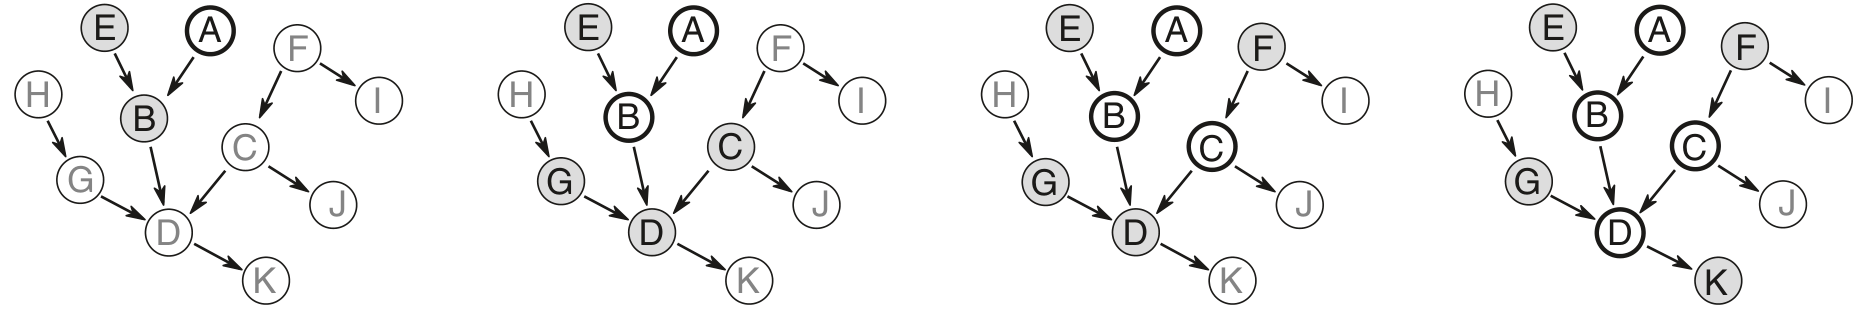
\includegraphics[scale=0.27]{../assets/greedy_mutex.png}
        
        \caption{Greedy expansion of $\{A\}$ (left to right).}
    \end{figure}
\end{example}

The \textit{proximity} $\delta(M)$ is utilized in line 2 of the algorithm to define the set of potential candidates that could expand $M$. Indeed, the goal of \textcite{mutex} is to identify mutually exclusive altered groups, where members share a \textbf{common downstream signaling target}. They state that this strategy narrows the search space to areas with a higher concentration of true positives. While it may slightly reduce \href{https://en.wikipedia.org/wiki/Precision_and_recall}{recall}, it also lessens the loss of statistical power associated with \href{https://en.wikipedia.org/wiki/Multiple_comparisons_problem}{multiple hypothesis testing}. Additionally, this approach provides an initial explanation for the observed mutual exclusivity, i.e. \textit{through a shared effect on a downstream gene}.

Another aspect to discuss is the \textit{null distribution} of a given gene $g \in M$, which represents $g$'s distribution under $H_0$ (defined in \cref{H_0}), denoted as $\mathcal N_g$ in the algorithm. Given a gene $g \in M$, \textcite{mutex} estimate $g$'s null distribution through a procedure that approximately involves the following steps:

\begin{enumerate}
    \item \textit{initialization}: define $\mathcal N_g$ as an empty list;
    \item \textit{iteration}: for $i = 1, \ldots, i_\mathrm{max}$ derive $\mathcal N_g \texttt{[}i\texttt{]}$ as follows:

        \begin{enumerate}
            \item randomly permute $g$'s alterations --- i.e., permute $g$'s column in $A$ randomly;
            \item let $M_g := \texttt{greedyMutex}(g, k_\mathrm{max}, G, A, \texttt{false})$;
            \item let $\mathcal P_g := \texttt{pValues}(M_g, A)$;
            \item let $\mathcal N_g \texttt{[}i\texttt{]} := \mathcal P_g\texttt{[}g\texttt{]}$.
        \end{enumerate}
\end{enumerate}

This is a \textit{sketch} of the complete procedure, and the omitted details extend well beyond the scope of this discussion. The main conclusion from this algorithm is that $g$'s \textit{null distribution} is derived from its $p$-value (namely $\mathcal P_g\texttt{[}g\texttt{]}$), computed when its alterations are randomly permuted. This randomization aims to modify $\inters$, simulating a scenario in which $H_0$ holds true, i.e. alterations in $\Gamma(g)$ are independent from mutations in $\Gamma(M - \{g\})$. Note that $\mathcal P_g\texttt{[}g\texttt{]}$ is computed through the \texttt{greedyMutex} function, with \texttt{final} set to \texttt{false} to prevent infinite recursion and avoid recomputing the \textit{null distributions}. In the \texttt{expandGroup} procedure, it will be assumed that for any $g \in M$, $\mathcal N_g$ can be computed as described.

With these definitions established, the \texttt{expandGroup} algorithm can be explained in detail. Specifically, it can be broken down into the following sections:

\begin{enumerate}
    \item if $\texttt{final} = \texttt{true}$, fill $\mathcal N$ such that $$\forall g \in M \quad \mathcal N \texttt{[}g\texttt{]} = \mathcal N_g$$ where $\mathcal N_g$ is $g$'s \textit{null distribution}, based on $g$'s $p$-value computed on $M$;
    \item \textit{initialization}: let $m_s$ be $M$'s \textit{score} (refer to \cref{score_mutex});
    \item \textit{iteration}: for each candidate $c$ in $\delta(M)$, compute as follows:
        \begin{enumerate}
            \item if $\texttt{final} = \texttt{true}$, update $\mathcal N$ such that $$\forall g \in (M \cup \{c\}) \quad \mathcal N \texttt{[}g\texttt{]} = \mathcal N_g'$$ where $\mathcal N_g'$ is $g$'s \textit{null distribution}, based both on $g$'s $p$-value computed on $M \cup \{c\}$, and on $\mathcal N_g$;
            \item let $c_s$ be $(M \cup \{c\})$'s score;
            \item if $c_s$ improves \textit{both} the current best score, and $m_s$, update the current best score with $c_s$.
        \end{enumerate}
    \item if the best candidate $b$ could be determined, return $M \cup \{b\}$; otherwise, return $M$.
\end{enumerate}

Note that this procedure requires $c_s$ to improve \textit{both} the current best score and $M$'s base score, meaning that suboptimal solutions are not explored by the algorithm.

Finally, the last procedure, which computes the mutual exclusivity score of a given gene set, can be introduced. Although this score is a crucial part of the metric developed by \textcite{mutex} to assess mutual exclusivity within a gene set, this algorithm could not be introduced in the previous chapter because it relies on the \textit{null distribution} dictionary $\mathcal{N}$, defined in \cref{expand_group_mutex}, which in turn depends on the \textit{null distribution} estimation, based on \cref{greedy_mutex} (with $\texttt{final} = \texttt{false}$).

\begin{algorithm}[H]
    \caption{
        \textit{Scoring procedure}: given a gene set $M$, a mutation matrix $A$, a boolean variable \texttt{final}, and a \textit{null distribution} dictionary $\mathcal N$, the algorithm computes $M$'s mutual exclusivity score.
    }

        \label{score_mutex}
    \begin{algorithmic}[1]
        \Function{score}{$M$, $A$, \texttt{final}, $\mathcal N$}
            \State $\mathcal P := \texttt{pValues}(M, A)$
            \If{$\texttt{final}$} \Comment{initial $p$-values correction}
                \For{$g \in M$}
                    % \State $c := 0$
                    \State $\mathcal N_g := \mathcal N\texttt{[}g\texttt{]}$
                    \State $c := \abs{\{i \mid \mathcal N_g\texttt{[}i\texttt{]} \le \mathcal P \texttt{[}g\texttt{]}\}}$
                    % \For{$i \in [1, \mathcal N_g.\texttt{len}()]$}
                    %     \If{$\mathcal N_g\texttt{[}i\texttt{]} \le \mathcal P\texttt{[}g\texttt{]}$}
                    %         \State $c \texttt{ += } 1$
                    %     \EndIf
                    % \EndFor
                    \State $\mathcal P\texttt{[}g\texttt{]} := \max\rbk{\mathcal P\texttt{[}g\texttt{]}, \dfrac{c}{\mathcal N_g.\texttt{len}()}}$
                \EndFor
            \EndIf
            \State \textbf{return} $\max_{g \in M}{\mathcal P\texttt{[}g\texttt{]}}$ \Comment{the \textit{least} significant is the \textit{largest}}
        \EndFunction
    \end{algorithmic}
\end{algorithm}

First, the algorithm evaluates $\mathcal P$, the $p$-value dictionary; then, if $\texttt{final} = \texttt{true}$, $\mathcal P$ is corrected for \textit{multiple hypothesis testing}. Finally, the largest value in $\mathcal P$ is returned. Note that both in line 7 and line 10, the largest value is chosen: this is because the \textit{larger} the $p$-value, the \textit{less significant} it is. Therefore, in line 7, the focus is on being as cautious as possible, while in line 10, the aim is to ensure that each member of $M$ contributes to the pattern. Lastly, the boolean variable \texttt{final} ensures that, during the evaluation of the \textit{null distributions}, the scores being used remain uncorrected.

The complete algorithm works by calling \texttt{greedyMutex} for each possible $g \in \mathcal G$ with \texttt{final} set to \texttt{true}, and then comparing the resulting sets. Finally, these sets may optionally undergo an \href{https://en.wikipedia.org/wiki/False_discovery_rate}{FDR} control procedure, which lies outside the scope of this work. Note that many details from the \href{https://github.com/PathwayAndDataAnalysis/mutex}{original code} have been removed for brevity, in each described algorithm.

\subsection{Results}

\textcite{mutex} applied their algorithm to identify mutual exclusion patterns in mutation and copy number profiles from multiple TCGA studies. The gene network they employed was cropped to the \textit{proximity} of significantly mutated genes (derived from MutSig \cite{mutsig}) and significantly altered genes (provided by GISTIC \cite{gistic}). Lastly, to reduce noise, genes with low alteration rates were filtered out in each study, and groups of up to 5 genes were examined.

They identified a total of 199 genes in their results, with 31 appearing in at least two studies. Notably, TP53 was the most recurrent gene, followed by well-known tumor suppressors and oncogenes such as PTEN, KRAS, and MYC. Among less recognized genes, \href{https://www.ncbi.nlm.nih.gov/gene/84033}{OBSCN} and \href{https://www.ncbi.nlm.nih.gov/gene/8289}{ARID1A} are highlighted for their potential roles in cancer --- the latter has previously been shown to act as a tumor suppressor in \href{https://en.wikipedia.org/wiki/Gastrointestinal_cancer}{gastrointestinal cancers} (GI). The most frequent common targets among the result groups include PIK3R1, HRAS, BRAF, MYC, RAC1, and \href{https://www.ncbi.nlm.nih.gov/gene/389}{RHOC}, with mutually exclusive alterations observed upstream of RHOC in five datasets. Although RHOC alterations are infrequent in TCGA samples, its overexpression is associated with cancer cell metastasis, suggesting that its activation may represent a significant downstream effect of driver alterations.

To assess the novelty of the findings, \textcite{mutex} examined co-citations of the recurrent genes with the term \curlyquotes{cancer}, using CoCiter. The last 10 genes on the list had fewer than 25 co-citations, indicating they are not well-established cancer drivers. However, further investigation revealed that 5 of these genes --- \href{https://www.ncbi.nlm.nih.gov/gene/8295}{TRRAP}, OBSCN, \href{https://www.ncbi.nlm.nih.gov/gene/6016}{RIT1}, \href{https://www.ncbi.nlm.nih.gov/gene/116986}{AGAP2}, and \href{https://www.ncbi.nlm.nih.gov/gene/6097}{RORC} --- contain so called \textit{mutation hotspots}. Mutation hotspots are DNA segments particularly prone to genetic alterations \cite{mutation_hotspot}, and are considered indicators of driver mutations, as changes in different regions of a driver gene can confer varying levels of selective advantage to a cancer cell --- passenger mutations are typically randomly distributed \cite{mutex}. Among the remaining 5 genes, the gene pair (\href{https://www.ncbi.nlm.nih.gov/gene/29956}{CERS2}, \href{https://www.ncbi.nlm.nih.gov/gene/23385}{NCSTN}) showed copy number alterations in the results.

Additionally, \textcite{mutex} compared the performance of their method with several previously published studies, including Dendrix \cite{dendrix}, MDPFinder \cite{mdpfinder}, and Multi-Dendrix \cite{multi-dendrix}. They derived a large dataset from breast cancer data in \href{https://www.cbioportal.org/}{cBioPortal}, which included 830 genes with an alteration rate of at least 3\% across 958 samples. This dataset was constructed through several steps aimed at randomizing gene alterations while preserving alteration ratios. Mutex outperformed the other methods, significantly improving the \href{https://en.wikipedia.org/wiki/Receiver_operating_characteristic}{receiver operating characteristic} (ROC) curves; notably, a modified version of Mutex that \textit{did not} use signaling networks showed decreased performance, highlighting the advantages of incorporating pathway information. In contrast, Dendrix, MDPFinder, and Multi-Dendrix performed poorly due to their reliance on the same weight function $W(M)$, which favors noise over signal. Moreover, other methods' generative models also struggled because they assumed equal alteration chances among group members. Mutex demonstrated improved scoring criteria and efficiency, exhibiting strong scalability in terms of memory and runtime, comparable to MDPFinder, and significantly more efficient than Dendrix and similar algorithms.

In conclusion, the greedy algorithm developed by \textcite{mutex} identified known mutually exclusive driver pathways, and highlighted potential roles for lesser-known genes, namely OBSCN, ARID1A and RHOC.

The following section will outline the different versions of the clustering algorithm, anticipated in the previous chapter.

\section{$\mathrm{C}^3$}

\subsection{Multiple versions}

In the final section of the previous chapter (namely, \cref{c3_chap2}), it was mentioned that \textcite{c3} developed multiple versions of their clustering algorithm; these variants will be explored in detail in the following paragraphs. In particular, they defined three methods for assigning weights to the edges of their gene graph $G$, to perform their vertex clustering algorithm, called $\mathrm{C}^3$ (\textit{knowledge-based} \cite{survey}):

\begin{enumerate}
    \item \textbf{ME-CO}, where $w^-$ depends on \textit{mutual exclusivity} and $w^+$ depends on \textit{coverage};
    \item \textbf{NI-ME-CO}, where $w^-$ depends on \textit{mutual exclusivity} and $w^+$ depends on \textit{coverage} and \textit{network information};
    \item \textbf{EX-ME-CO}, where $w^-$ depends on \textit{mutual exclusivity} and $w^+$ depends on \textit{coverage}, and \textit{expression data}.
\end{enumerate}

Note that $w^-$ depends solely on the mutual exclusivity component in each version of the algorithm, whereas the value of $w^+$ depends on the chosen algorithm variant. The following section will introduce the standard version of $\mathrm{C}^3$.

\subsection{The standard version}

The initial version of their clustering algorithm is the standard one, which considers only \textbf{mutual exclusivity} and \textbf{coverage}, and it is described below.

\begin{definition}[ME-CO]
    In the \textbf{ME-CO} version of the algorithm, the following definitions apply:

    \begin{equation}
        \forall u, v \in V(G) \quad w_{uv}^- := w^-_{uv}(\mathrm e)
    \end{equation}

    \begin{equation}
        \forall u, v \in V(G) \quad w_{uv}^+ := w^+_{uv}(\mathrm c)
    \end{equation}
\end{definition}

The definitions for $w_{uv}^-(\mathrm e)$ and $w_{uv}^+(\mathrm c)$ are provided in \cref{me_comp} and \cref{co_comp} respectively.

Note that in each variation discussed, optional rescaling is applied to ensure that the weight formulas satisfy additional constraints required later in the algorithm, though the specifics are beyond the scope of this analysis.

While this version of the algorithm does not include any external data, the variant outlined in the next section incorporates additional supplementary information into the weights.

\subsection{Integrating network information}

Pan-cancer studies, as reported in multiple papers, have demonstrated a significant relationship between network topology and the distribution patterns of cancer drivers. Specifically, the impact of deleterious mutations on the phenotype can be mitigated by certain configurations of the corresponding protein complexes, while other arrangements can amplify their effect. For example, most variants found in healthy individuals tend to be located at the periphery of the interactome, where they do not affect network connectivity. In contrast, cancer-driver somatic mutations are more likely to occur in central, internal regions of the interactome and within highly integrated components \cite{c3}. This suggests that network topology significantly influences the impact of cancer driver mutations, and to assess the implications for cancer development, \textcite{c3} analyzed network distances between driver variants to identify patterns.

To precisely quantify the network distances between driver variants, \textcite{c3} computed the pairwise network distances between genes within a large pathway, comprising 8726 genes, by using an implementation of the standard \href{https://en.wikipedia.org/wiki/Dijkstra%27s_algorithm}{Dijkstra algorithm}. To reduce the computational cost of running Dijkstra's algorithm $O\rbk{8726^2}$ times, 1000 pairs were randomly selected for this test. Using the most comprehensive known driver list from the Cancer Gene Census (CGC) \cite{cgc}, the same distances were calculated for driver genes, this time for all gene pairs. The resulting distribution of shortest paths is shown in \cref{frequency_c3} \cite{c3}, revealing that the average shortest distance between drivers is \textit{significantly smaller} than that between two randomly selected genes.

\begin{figure}[H]
    \centering
    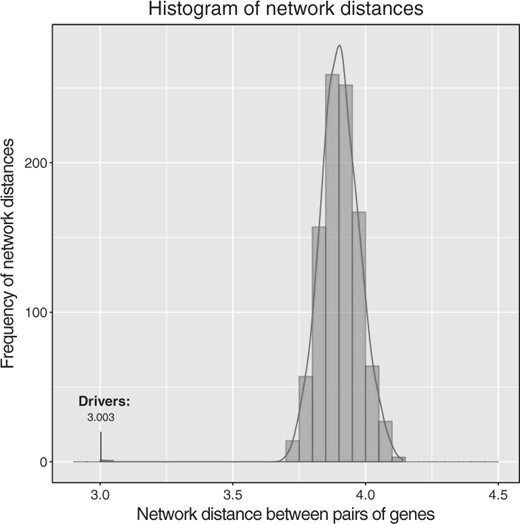
\includegraphics[scale=0.6]{../assets/frequency_c3.jpeg}
    
    \caption{Distribution of distances between genes in the network.} \label{frequency_c3}
\end{figure}

These findings indicate that network distance and connectivity information should be considered when identifying potential driver mutations. This can be achieved by adjusting the positive weight of edges connecting two genes: specifically, if both endpoint genes are drivers, they should be sufficiently central within a given pathway, close to other known drivers, or to each other.

Hence, from the KEGG \cite{kegg} database, \textcite{c3} built an undirected graph $G'$, where each vertex represents a gene and the edges describe interactions between them --- note that $\abs{V(G)} = \abs{V \left(G' \right)} = n$. For each vertex $u \in V \left(G' \right)$, let $\mathscr{N}(u)$ denote the set of $u$'s neighbors, and let $\mathscr{N}'(u) := \mathscr{N}(u) \cup \{u\}$. Also, let

\begin{equation}
    f(u, v) := \dfrac{\abs{\mathscr{N}'(u) \cap \mathscr{N}'(v)}}{\abs{\mathscr{N}'(u) \cup \mathscr{N}'(v)}}
\end{equation}

which is referred to as the \href{https://en.wikipedia.org/wiki/Jaccard_index}{Jaccard similarity coefficient}; a large value of $f(u, v)$ indicates that $u$ and $v$ are well connected in $G'$ and are likely involved in the same pathway, suggesting that they should be clustered together. Furthermore, let

\begin{equation}
    \mathscr{F} := \{f(u, v) \mid u, v \in V\rbk{G'}\}
\end{equation}

and let $T'(J')$ be the $J'$-th percentile of the values in $\mathscr F$.

The network information component of the positive weights is described below.

\begin{definition}[Network information component]
    The \textbf{network information component} is defined as follows: $$w_{uv}^+(\mathrm n) := \soe{ll}{1 & f(u, v) > T'(J') \\ \dfrac{f(u, v)}{T'(J')} & f(u, v) \le T'(J')}$$
\end{definition}

Finally, the version of $\mathrm{C}^3$ that incorporates the network information is defined as follows.

\begin{definition}[NI-ME-CO]
    The \textbf{NI-ME-CO} version of the algorithm is defined by the following equations:

    \begin{equation}
        \forall u, v \in V(G) \quad w_{uv}^- := w_{uv}^-(\mathrm e)
    \end{equation}

    \begin{equation}
        \forall u, v \in V(G) \quad w_{uv}^+ := w_1 w_{uv}^+(\mathrm c) + w_2 w_{uv}^+(\mathrm n)
    \end{equation}

    where $w_1, w_2 \ge 0$ and $w_1 + w_2 = 1$.
\end{definition}

The next section will describe a third variant, that incorporates gene expression data instead of network information.

\subsection{Integrating expression data}

Another valuable type of data that could be integrated into the positive weights for clustering is \textbf{gene expression data}. This is based on the assumption that co-expressed genes are likely to be involved in the same function or cancer pathway. Therefore, genes with strong positive or negative co-expression should be clustered together. The following paragrpahs will describe how \textcite{c3} include expression data into $w^+$.

Given a vertex $u \in V(G)$, let $\mathrm {\mathbf z(u)}$ be the vector of the time-evolving expression values of $u$ \todo{la prima volta che lessi questo paper non trovai niente sul dove presero queste informazioni, e tutt'ora non mi pare che lo menzionino da nessuna parte; scrivono solo che le informazioni le prendono dal TCGA e dal KEGG, suppongo a questo punto che queste info siano ottenibili dal TCGA ma dovrei controllare manualmente}. Thus, let

\begin{equation}
    g(u, v) := \dfrac{\abs{\abk{\mathrm{\mathbf z(u)}, \mathrm{\mathbf z(v)}}}}{\abs{\abs{\mathrm{\mathbf z(u)}}} \abs{\abs{\mathrm{\mathbf z(v)}}}}
\end{equation}

where $\abk{\mathrm{\mathbf a}, \mathrm{\mathbf b}}$ denotes the inner product of the vectors $\mathrm{\mathbf a}$ and $\mathrm{\mathbf b}$, while $\abs{\abs{\mathrm{\mathbf a}}}$ stands for its $L^2$ norm. This equation is known as the \href{https://en.wikipedia.org/wiki/Cosine_similarity}{cosine similarity}, since the ratio that defines $g(u, v)$ is equal to the cosine of the angle between $\mathrm {\mathbf z(u)}$ and $\mathrm {\mathbf z(v)}$ --- the only difference being the absolute value in the numerator, to capture both positive and negative correlations. A large value of $g(u, v)$ suggests that the expression vectors of $u$ and $v$ are highly correlated, hence they should be clustered together. Note that $$\forall u, v \in V(G) \quad 0 \le g(u, v) \le 1$$ Moreover, let

\begin{equation}
    \mathscr G := \{g(u, v) \mid u, v \in V(G)\}
\end{equation}

and let $T''(J'')$ be the $J''$-th percentile of the values in $\mathscr G$.

Hence, the gene expression component of the positive weights can be defined as follows.

\begin{definition}[Expression data component]
    The \textbf{expression data component} is defined as follows: $$w_{uv}^+(\mathrm x) := \soe{ll}{1 & g(u, v) > T''(J'') \\ \dfrac{g(u, v)}{T''(J'')} & g(u, v) \le T''(J'')}$$
\end{definition}

Lastly, the third variant of $\mathrm{C}^3$ is described below.

\begin{definition}[EX-ME-CO]
    The \textbf{EX-ME-CO} version of the algorithm is defined by the following equations:

    \begin{equation}
        \forall u, v \in V(G) \quad w_{uv}^- := w_{uv}^-(\mathrm e)
    \end{equation}

    \begin{equation}
        \forall w_{uv}^+ := w_1 w_{uv}^+(\mathrm c) + w_2 w_{uv}^+(\mathrm x)
    \end{equation}

    where $w_1, w_2 \ge 0$ and $w_1 + w_2 = 1$.
\end{definition}

\subsection{Other versions}

\textcite{c3} also mention that other combinations can be used, with appropriate adjustments to the weights, such as the following version, which will be referred to as NI-EX-ME-CO in this work.

\begin{definition}[NI-EX-ME-CO]
    The \textbf{NI-EX-ME-CO} version of the algorithm is defined by the following equations:

    \begin{equation}
        \forall u, v \in V(G) \quad w_{uv}^- := w_{uv}^-(\mathrm e)
    \end{equation}

    \begin{equation}
        \forall w_{uv}^+ := w_1 w_{uv}^+(\mathrm c) + w_2 w_{uv}^+(\mathrm n) + w_3 w_{uv}^+(\mathrm x)
    \end{equation}

    where $w_1, w_2, w_3 \ge 0$ and $w_1 + w_2 + w_3 = 1$.
\end{definition}

The previous sections outlined the definition of the weights for the edges in the gene graph $G$; instead, the following ones will explain how $\mathrm{C}^3$ operates.

\subsection{The clustering ILP} \label{the_clustering_ilp}

\textcite{c3} opted to use an ILP approach to formulate the clustering algorithm, utilizing the weights defined in the previous sections.

Note that the classical formulation of correlation clustering does not impose any restrictions on cluster sizes. However, most driver identification methods inherently include cluster size limits, as they directly affect the computational complexity of the algorithms --- many even fail to operate beyond a certain size. Another reason for imposing a cluster size limit is the expectation that driver genes of specific cancer types will be grouped together, and recent findings indicate that only a small number of drivers are typically present in any given cancer type. Thus, if clusters are too large, they may include drivers from multiple cancer types, hiding this separation of the drivers. Furthermore, introducing cluster size constraints helps to avoid the formation of non-informative \textit{giant clusters} or \textit{singleton clusters} \cite{c3}.

Therefore, \textcite{c3} introduce a cluster size constraint by assuming that all clusters are of size $k$ at most; clearly, setting $k$ equal to the total number of vertices effectively removes this constraint, allowing flexibility in cluster size selection.

The ILP of $\mathrm{C}^3$ is defined as follows.

\begin{definition}[$\mathrm{C}^3$'s ILP] \label{c3_ilp}
    The \textbf{$\mathrm{C}^3$ algorithm} can be defined by the following ILP:

    \begin{equation} \label{c3_first}
        \mathrm{minimize} \sum_{e \in E(G)} (w_e^+x_e + w_e^-(1 - x_e)),
    \end{equation}

    \begin{equation} \label{c3_second}
        \mathrm{subject \ to \ } x_{uv} \le x_{uz} + x_{zv}, \quad u, v, z \in V(G) \mathrm{\ distinct},
    \end{equation}

    \begin{equation} \label{c3_third}
        \sum_{v \in V(G) \atop u \neq v} (1 - x_{uv}) \le k, \quad u \in V(G),
    \end{equation}

    \begin{equation} \label{c3_fourth}
        x_e \in \{0, 1\}, \quad e \in E(G).
    \end{equation}
\end{definition}

In this formulation, the variables $x_e$ allow to describe any clustering of the vertices of $G$, since $x_e \in \{0, 1\}$ for each $e \in E(G)$.

Note that \cref{c3_first} aligns with the definition provided in \cref{c3_chap2}, as $x_{uv} = 1$ implies that $u$ and $v$ should belong to different clusters, while $x_{uv} = 0$ implies that the two vertices should be placed into the same cluster.

Furthermore, \cref{c3_third} states that for a fixed vertex $u \in V(G)$, the number of variables $x_{uv}$ equal to 0, for any $v \in \mathcal N(u)$, must not exceed $k$ --- which is the clustering size constraint previously discussed.

Lastly, \cref{c3_second} is the \href{https://en.wikipedia.org/wiki/Triangle_inequality}{triangle inequality}, which ensures that if $u$ and $z$ are placed in the same cluster, and $z$ and $v$ are also placed in the same cluster, then $u$ and $v$ will be clustered together. This means that \textit{belonging to the same cluster is a transitive property}, since $$\soe{l}{x_{uz} = 0 \\ x_{zv} = 0 \\ x_{uv} \le x_{uz} + x_{zv}} \implies x_{uv} = 0$$

The next section will illustrate a relaxation of this ILP.

\subsection{The rounding procedure}

Since solving binary ILPs is \NPComplete \cite{karp}, \textcite{c3} relax the problem by changing \cref{c3_fourth} to an interval constraint $$0 \le x_e \le 1$$ leading to an LP program, the solution of which may be fractional. Hence, to obtain a valid clustering, the fractional solutions have to be rounded. Therefore, instead of solving the LP, they remove \cref{c3_third} from the linear program, and employ the following rounding procedure to round the fractional values.

\begin{algorithm}[H]
    \caption{
        \textit{Rounding procedure}: given a solution $\{x_e\}_{e \in E(G)}$ of the relaxed version of the ILP provided \cref{c3_ilp}, a rational value $\alpha$, and the maximum cluster size $k$, the algorithm rounds the solution to integer values.
    }

        \label{rounding_procedure}
    \begin{algorithmic}[1]
        \Function{roundingProcedure}{$G$, $\{x_e\}_{e \in E(G)}$, $\alpha$, $k$}
            \State $\mathcal C := \varnothing$ \Comment{the output set of clusters}
            \State $S := V(G)$
            \While{$S \neq \varnothing$}
                \State Choose an arbitrary $u \in S$ \Comment{this is the \textit{pivot vertex}}
                \State $T := \{w \in S - \{u\} \mid x_{uw} \le \alpha\}$ \Comment{$u$'s neighbors under $\alpha$'s threshold}
                \If{$\sum_{w \in T}{x_{uw}} \ge \frac{\alpha}{2}\abs{T}$}
                    \State $\mathcal C = \mathcal C \cup \{\{u\}\}$ \Comment{add a singleton cluster $\{u\}$}
                    \State $S = S - \{u\}$
                \ElsIf{$\abs{T} \le k$}
                    \State $\mathcal C = \mathcal C \cup \{\{u\} \cup T\}$ \Comment{add the cluster $(\{u\} \cup T)$}
                    \State $S = S - \rbk{\{u\} \cup T}$
                \Else
            \State Partition $T$ into $\{T_0', T_1, \ldots, T_p\}$, such that: \begin{itemize} \item[] \quad \quad \quad \quad $\sbullet \ \abs{T_0'} = k$ \item[] \quad \quad \quad \quad $\sbullet \ \abs{T_i} = k + 1$ for each $0 < i < p$ \item[] \quad \quad \quad \quad $\sbullet \ \abs{T_p} \le k + 1$ \end{itemize}
                    \State $T_0 := T_0' \cup \{u\}$ \Comment{$T_0$ has $k + 1$ elements}
                    \For{$i \in [0, p]$}
                        \State $\mathcal C = \mathcal C \cup \{T_i\}$ \Comment{add each partition as a cluster}
                    \EndFor
                    \State $S = S - \rbk{\{u\} \cup T}$
                \EndIf
            \EndWhile
            \State \textbf{return} $\mathcal C$
        \EndFunction
    \end{algorithmic}
\end{algorithm}

The algorithm can be summarized as follows:

\begin{enumerate}
    \item \textit{initialization}: let $\mathcal C := \varnothing$ and $S := V(G)$;
    \item \textit{iteration}: while $S \neq \varnothing$, compute as follows:
        \begin{enumerate}
            \item choose a \textit{pivot} vertex $u \in S$ arbitrarily;
            \item let $T$ be the set of $u$'s neighbors $w \in \mathcal N (u)$ such that $x_{uw}$ is at most $\alpha$;
            \item if $\frac{\alpha}{2} \abs{T}$ is at most $\sum_{w \in T}{x_{uv}}$, add $\{u\}$ to $\mathcal C$ as a \textit{singleton cluster}, and remove $u$ from $S$;
            \item otherwise, if $\abs{T}$ is at most $k$, add $\{u\} \cup T$ to $\mathcal C$ as a cluster, and remove it from $S$;
            \item otherwise, partition $T$ in multiple subsets, such that each subset contains $k + 1$ elements (technically, the last partition will contain only the remaining elements), and the first subset contains $u$; then, add each partition of $T$ as a separate cluster to $\mathcal C$, and remove every partition from $S$.
        \end{enumerate}
\end{enumerate}

The rationale behind the condition in line 7 can be elucidated by examining the meaning of $x_{uw}$: specifically, if $x_{uw}$ is close to 1, $u$ and $w$ are likely to be placed in different clusters, as previously described \cref{the_clustering_ilp}. Note that, if the sum $\sum_{w \in T}{x_{uw}}$ is greater than or equal to a value proportional to $\abs T$, it indicates that there are numerous edges $(u, w)$ for $w \in T$ with significantly high $x_{uw}$. Therefore, this suggests that $u$ should likely be placed in a cluster distinct from all its \textit{filtered} neighbors $T$.

In contrast, if this condition does not hold, it is probable that several variables indicate that $u$ should be clustered with some of its \textit{filtered} neighbors. Therefore, when this condition fails, and $\abs T \le k$, $u$ and $T$ are forced to form a cluster in line 11.

Lastly, if none of the preceding conditions are satisfied, it means that $u$ should not form a \textit{singleton cluster}, but the presence of numerous \textit{filtered} neighbors precludes the formation of a $T \cup \{u\}$ cluster. Therefore, line 14 partitions $T$ into smaller clusters of size $k + 1$.

As a final note, \textcite{c3} conducted an analysis to determine the optimal value for $\alpha$, which was found to be $\frac{2}{7}$, but the proof of this value is beyond the scope of this work.

Finally, the complete $\mathrm{C}^3$ algorithm that \textcite{c3} employed to obtain their results is described below.

\begin{definition}[$\mathrm{C}^3$] \label{c3_final}
    The \textbf{$\mathrm{C}^3$ algorithm} is defined as follows: first, the next ILP is solved

    \begin{equation}
        \mathrm{minimize} \sum_{e \in E(G)} (w_e^+x_e + w_e^-(1 - x_e)),
    \end{equation}

    \begin{equation}
        \mathrm{subject \ to \ } x_{uv} \le x_{uz} + x_{zv}, \quad u, v, z \in V(G) \mathrm{\ distinct},
    \end{equation}

    \begin{equation}
        0 \le x_e \le 1, \quad e \in E(G).
    \end{equation}

    and then the rounding procedure defined in \cref{rounding_procedure} is applied.
\end{definition}

\subsection{Results}

placeholder \todo{todo todo}

\cleardoublepage
